\section{approach}
\label{sec:approach}
In this section, we first formulate the just-in-time defect prediction and provide an overview of our framework. We then describe the details of each part inside the framework. Finally, we present an algorithm for learning effective settings of our model's parameters. 
\subsection{Framework Overview}
\label{sec:overview}

\begin{figure}
\center
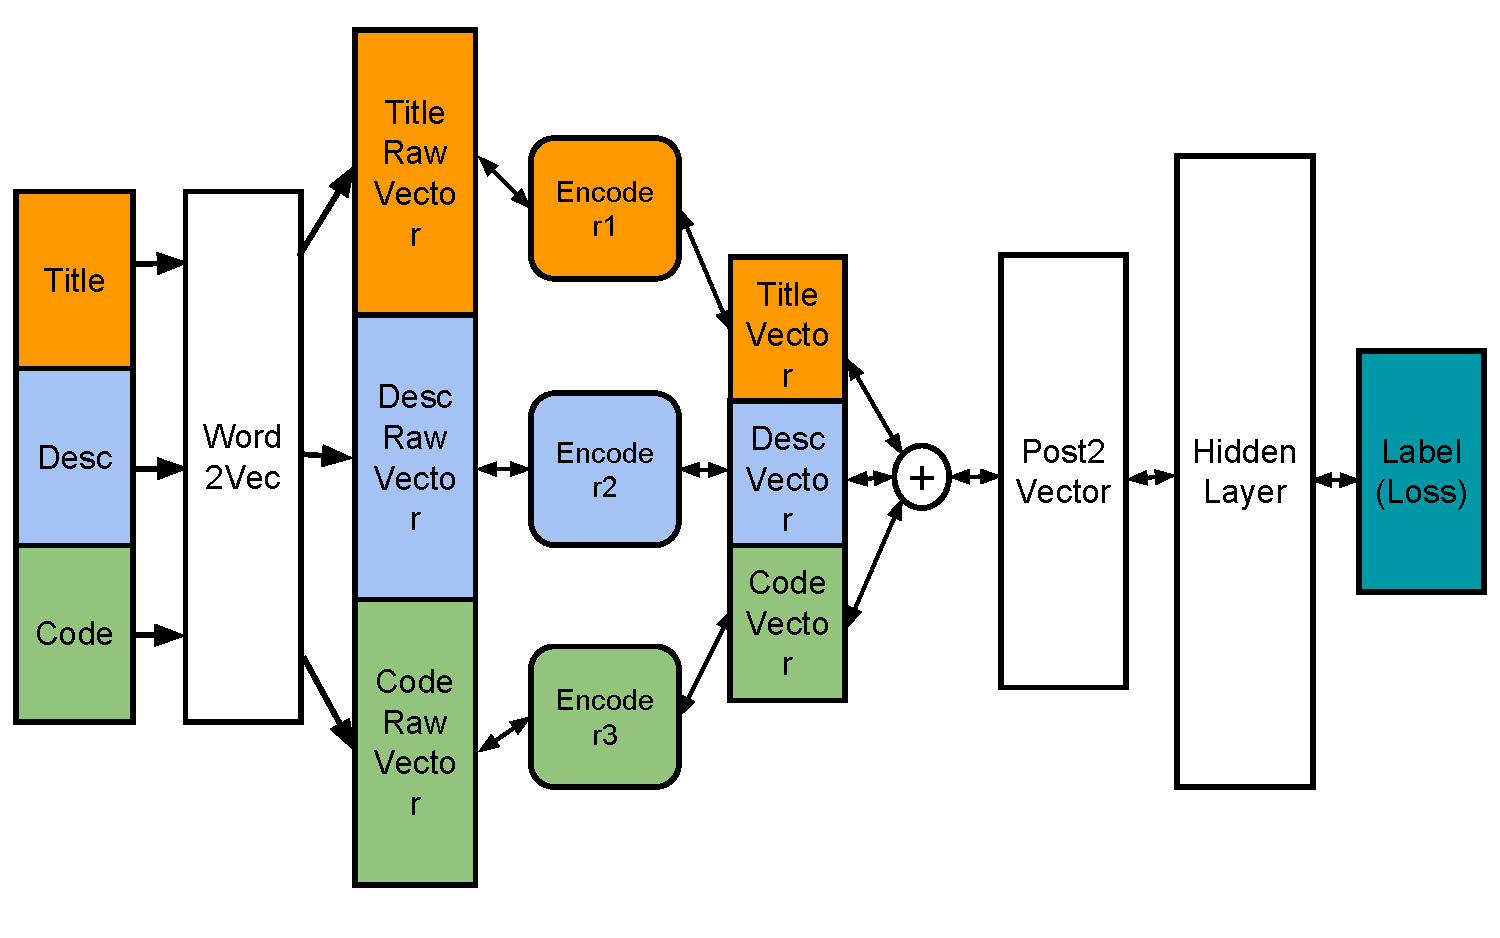
\includegraphics[scale=0.36]{figs/framework.pdf}
\caption{The general framework of just-in-time defect prediction model.}
\label{fig:overview}
\end{figure}

The goal of the just-in-time defect prediction model is to automatically label a commit change as bug or clean to help developers better focus on their efforts on assuring software quality. We consider the just-in-time defect prediction problem as a learning task to construct prediction function $\textbf{f}:
\mathcal{X} \longmapsto \mathcal{Y}$, where $y_i \in \mathcal{Y} = \{0, 1\}$ indicates whether a commit change $x_i \in \mathcal{X}$ cleans ($y_i = 0$) or contains a buggy code ($y_i = 1$). The prediction function $\textbf{f}$ can be learned by minimizing the following objective function:
\begin{equation}
\underset{\textbf{f}}{min} \sum_{i}\mathcal{L}(\textbf{f}(x_i), y_i) + \lambda\Omega(\textbf{f})
\end{equation}
where $\mathcal{L}(.)$ is the empirical loss function measuring the difference between the predicted and the output label, $\Omega(\textbf{f})$ is a regularization function to prevent the over fitting problem, and $\lambda$ the trade-off between $\mathcal{L}(.)$ and $\Omega(\textbf{f})$. Figure~\ref{fig:overview} illustrates the overview framework of the just-in-time defect prediction model. The model consists of four parts: input layer, feature extraction layer, feature combination layer, and the output layer. We explain the details of each part in the following subsections.

\subsection{Input Layer}
\label{sec:input_layer}
To feed the raw textual data to convolutional layers for feature learning, we first encode a commit message and code changes in the input layer. We represent each word in the commit message and code changes as $d$-dimensional vector. After the preprocessing step, the $\mathcal{X}^{m}_i$ and $\mathcal{X}^{c}_i$, which are the encoded data of the commit message and code changes respectively, are passed to the convolutional layers to extract the commit message and code changes features. In the convolutional layers, the commit messages and code changes are processed independently to extract the features based on each type of textual information. These features from the commit messages and code changes are then combined into a unified feature representation, and followed by a linear hidden layer connected to output layer used to produce the output label $\mathcal{Y}$ indicating whether the commit change $x_i$ cleans or contains a buggy code. 

The novelty of the just-in-time defect prediction model lies in the convolutional network layers for code changes and the feature combination layers. In the following subsection, we firstly discuss the convolutional layers for the commit message and present the novelty of our model in more details. 

\subsection{Convolutional Network Architecture for Commit Message}
\label{sec:cnn_msg}
The underlying deep neural network for commit message is a Convolutional Neural Network (CNN). CNN firstly used to automatically learn the salient features in the images from raw pixel values~\cite{krizhevsky2012imagenet}. However, CNN has been also used a lot and showed extraordinary successes in Natural Language Processing (NLP)~\cite{kim2014convolutional, dos2014deep, kalchbrenner2014convolutional, zhang2015character, johnson2014effective}. The architecture of CNN allowed it to extract the structural information features from raw text data of word embedding. Next, we describe how a simple CNN can be used to learn the commit message's features.

Given a commit message $\textbf{m}$ which is essentially a sequence of words $[w_1, \dots, w_{|m|}]$. We aim to obtains its matrix representation $\textbf{m} \rightarrow \textbf{M} \in \mathbb{R}^{|m| \times d_m}$, where the matrix $\textbf{M}$ comprises a set of words $w_i \rightarrow W_i$, $i = 1, \dots, |m|$ in the given commit message. Each word $w_i$ now is represented by an embedding vector, i.e., $W_i \in \mathbb{R}^{d_m}$, where $d_m$ is a $d_m$-dimensional vector of a word appearing in the commit message. 

Following the previous works~\cite{kim2014convolutional, zhang2015character}, the $d_m$-dimensional representing an embedding vector extracted from an embedding matrix which is randomly initialized and jointly learned with the CNN model. In our paper, the embedding matrix of commit message is randomly initialized and learned during the training process. Hence, the matrix representation $\textbf{M}$ of the commit message $\textbf{m}$ with a sequence of $|m|$ words can be represented as following:
\begin{equation}
\label{eq:representation_msg}
    \textbf{M} = [W_1, \dots, W_{|m|}]
\end{equation}
For the purpose of parallelization, all commit messages are padded or truncated to the same length $|m|$. 

To extract the commit message's salient features, a filter $f \in \mathbb{R}^{k \times {d_m}}$, followed by a non-linear activation function $\alpha (.)$, is applied to a window of $k$ words to produce a new feature as following:
\begin{equation}
\label{eq:filter_msg}
    c_i = \alpha(f * M_{i:i+k-1} + b_i)
\end{equation}
where $*$ is a sum of element-wise product, and $b_i \in \mathbb{R}$ is the bias value. In our paper, we choose the rectified linear unit (RELU) as our activation function since it achieved a better performance compared to other activation functions~\cite{nair2010rectified, dahl2013improving, he2016deep}. The filter $f$ is applied to every $k$-words of the commit message, these outputs of this process are then concatenated to product output vector $\textbf{c}$ such that:
\begin{equation}
\label{eq:output_ftr_msg}
\textbf{c} = [c_1, \dots, c_{|m| - k + 1}]
\end{equation}

By applying the filter $f$ on every $k$-words of the commit message, the CNN is able to exploit the semantic information of its input. In practice, the CNN model may include multiple filters with different $k$. These hyperparameters need to be set by the user before starting the training process. To characterize the commit message, we apply a max pooling operation~\cite{lecun2015deep} over the output vector $\textbf{c}$ to obtain the highest value as following: 

\begin{equation}
\label{eq:max_pooling_msg}
\underset{1 \leq i \leg |m| - k + 1}{max} c_i
\end{equation}

The results of the max pooling operation from each filter are then used to form an embedding vector (i.e., $z_\textbf{m}$) of the commit message (see Figure~\ref{fig:overview}). 

\subsection{Convolutional Network Architecture for Code Changes}
\label{sec:cnn_code}
In this section, we focus on building convolutional networks for code changes to solve the just-in-time defect prediction problem. 

Code changes, although it can be viewed as a sequence of words, differs from natural language mainly because of its structure. The natural language carries sequences of words, and the semantics of the natural language can be inferred from a bag of words~\cite{ng1997corpus}. On the other hand, the code changes includes a change in different files and different kinds of changes (removals or additions) for each file. Hence, to extract silent features from the code changes, the convolutional networks should obey the code changes structure. 


